%\documentclass[12pt]{scrreprt}
\documentclass[12pt]{report} 

% language may be romanian or english (default is english)
% type may be bachelor or master (default is bachelor)
\usepackage[language=english, type=bachelor]{style}
\usepackage{amsmath}

%\geometry{a4paper,top=2.5cm,left=3cm,right=2.5cm,bottom=2.5cm}
%in style
%controlling the appearance of your headers and footers
\usepackage{fancyhdr}
\pagestyle{fancy}
\lhead{}
\chead{}
\renewcommand{\headrulewidth}{0.2pt}
\renewcommand{\footrulewidth}{0.2pt}

\begin{document}

\specialization{COMPUTER SCIENCE ROMANIAN}	
\title{Depression signs detection}					   
\author{Dinica Mircea}											
\supervisor{Lector Universitar, Lupea Mihaiela}				
				
\maketitle


\newpage
\thispagestyle{empty}
\mbox{}
\newpage
\pagenumbering{roman} 

\cleardoublepage
ABSTRACT
\vspace{0.5cm}	
\hrule
\vspace{0.5cm}	
%\cleardoublepage

The purpose of this paper is to research the viability of machine translation of text from English to Romanian, in order to use Natural Language Processing(NLP) and Artificial Intelligence(AI) in order to detect if the text shows signs of depression or not. Depression is a major problem right now, which if not addressed can cause serious problems. With the help of NLP and AI, it is desired to develop a tool for giving an opportunity to its users to have an easy way to get an initial assessment of their texts, in cases such as private text messages, their own thoughts or even help professionals reach possible clients in order to help them.

This paper describes its content in six chapters. Chapter 1 provides the motivation and purpose of the depression detection application. Chapter 2 gives details regarding the dataset used and the pre-processing techniques, namely BERT Tokenization and Linguistic Word Inquiry and Word Count which recognizes the emotions and grammar parts which the tokens belong to. Chapter 3 describes the machine learning classification algorithm Random Forest and the reason why it was chosen, and also the results of the training. Chapter 4 details the results of making a similar AI model for Romanian, which contains the tasks of translating the dataset, using the same pre-processing techniques and training the Random Forest algorithm.
Chapter 5 summarizes the architecture and technologies used to implement the practical tool. The final chapter outlines the conclusions and proposes future development ideas. 

As a practical tool for the algorithm, a web application which expects as input a text. The output is the class which was attributed to the text with a corresponding message advising the user to investigate further with the author of the text, and also the top 5 categories of words found in the input with their respective percentages related to total word count. This will be computed on a web back-end server, respecting the REST architectural style. The chosen technologies for developing the tool are Python with Flask framework for the back-end server and React, the JavaScript library for the front-end server.

\tableofcontents


\newpage
\pagenumbering{arabic}

\chapter{Introduction}

%\chapter*{Introduction}
\label{intro}

% \par Introducere: obiectivele lucrarii si descrierea succinta a capitolelor, prezentarea temei, prezentarea contributiei proprii, respectiv a rezultatelor originale si mentionarea (daca este cazul) a sesiunii de comunicari unde a fost prezentata sau a revistei unde a fost publicata.
%THEME PRESENTATION
\section{Depression Statistics and Insights}
\label{sec:ch1sec1}

\par \quad Depression stands as a mental health affliction with profound impacts on both psychological and physical well-being. Characterized by a disinterest in routine activities, sleep disturbances, anhedonia, and in severe cases, suicidal ideation \cite{cui2015systematic}, it has become a problem across worldwide. Furthermore, individuals with major depressive disorder face a bigger risk of cardiovascular problems, not optimal treatment outcomes, and higher rates of morbidity and mortality \cite{seligman2015interface,luo2018effects}.

The World Health Organization (WHO) identifies depression as the primary contributor to global disability, affecting over 300 million individuals worldwide \cite{smith2014world}. Particularly alarming is the revelation that adolescents with severe depression are 30 times more prone to suicide \cite{stringaris2017depression}. 
Although we know depression is a big problem worldwide, we still don't fully understand what causes it. We know that cultural, psychological, and biological factors play a part, but we don't know exactly how they all fit together.\cite{gross2014silver,menard2016pathogenesis}.

The Global Burden of Disease (GBD) study \cite{liu2020changes} offers comprehensive insights into various mental problems across 195 countries, including depression. Divided into dysthymia and major depressive disorder categories, the GBD database from 1990 to 2017 furnishes valuable data for understanding depression's evolution globally. Major depressive disorder emerges as a predominant form of depression, posing a significant burden on global health, indicating it may become the leading cause of disability by 2030. Moreover, while dysthymia rates decreased in some regions, it remains a concern, particularly in the United States.

Identifying underlying causes and risk factors for depression, including genetic predisposition, demographic factors, unhealthy lifestyles, and diseases coming from it such as stroke, cancer, and AIDS, highlights the need for a change. Governments in countries with high depression rates are encouraged to prioritize research, promote healthy lifestyles, and ensure comprehensive care for individuals with predisposing conditions. However, the study acknowledges limitations in data analysis, advocating for future research of regional risk factors and guide tailored policy interventions for effective depression control globally. This can be seen in Figure \ref{FigGloablDepression} \cite{liu2020changes}, which evaluated the worldwide burden of depression using the estimated annual percentage change (EAPC) and age-standardized incidence rate (ASR).

\begin{figure}[htbp]
	\centering
		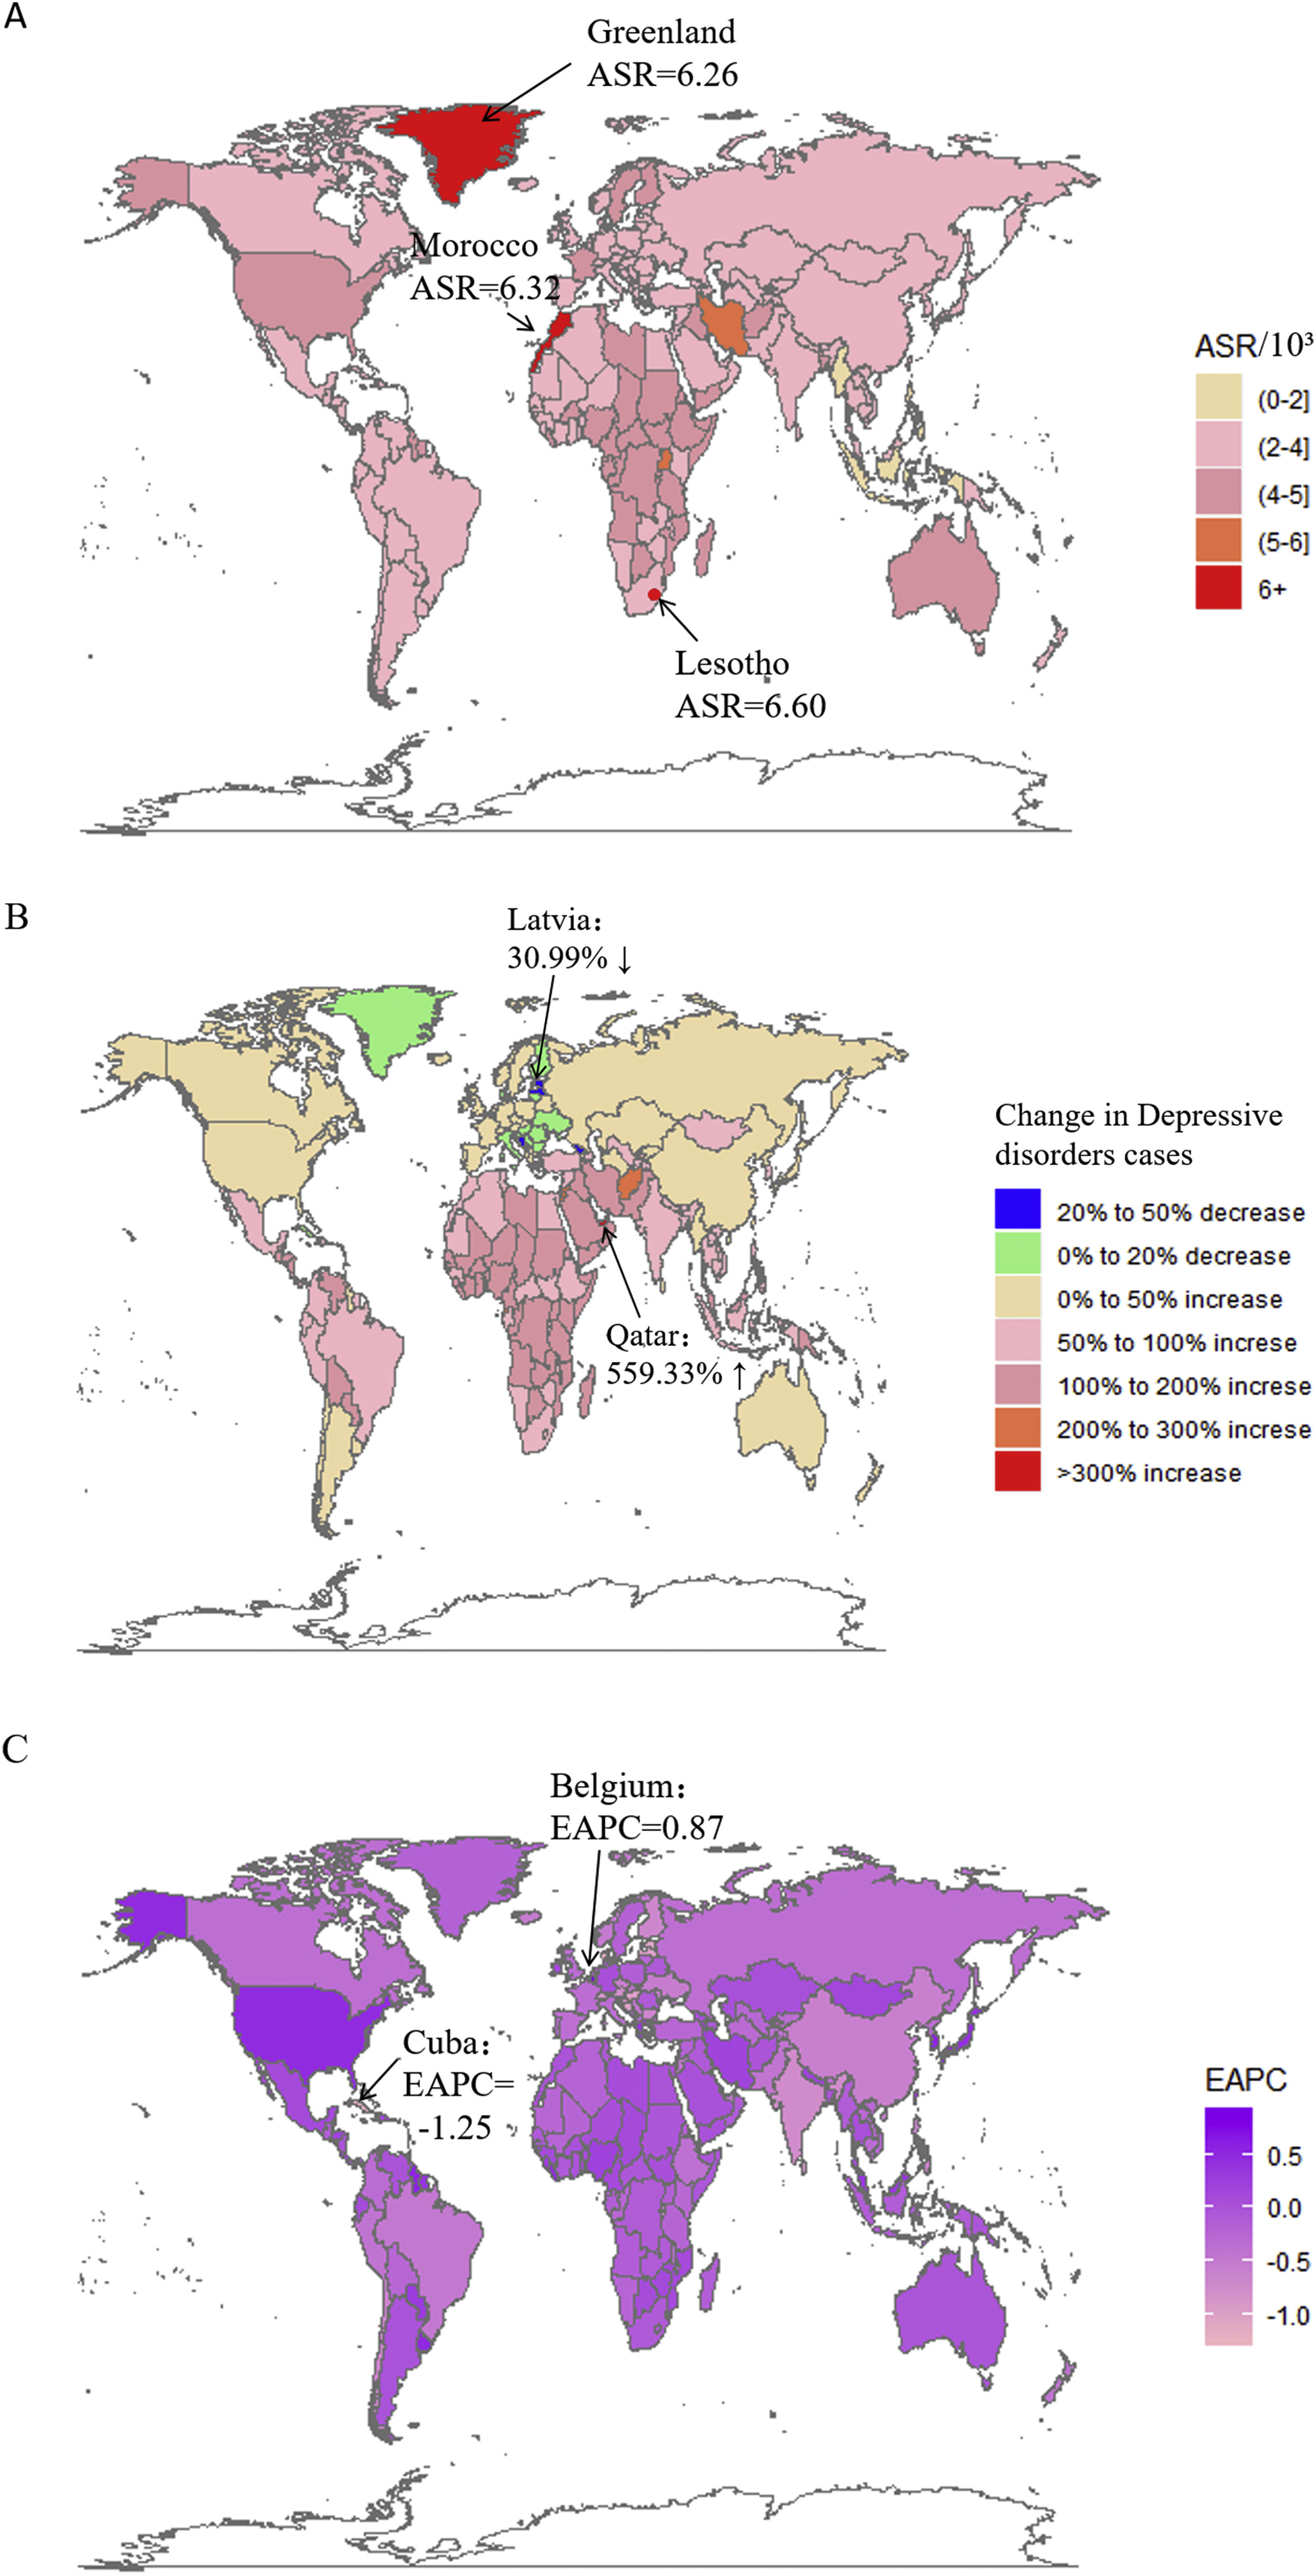
\includegraphics[scale=0.65]{./figures/depression-map-Liu-et-al-2020.jpg}
	\caption{Global depression statistics comparison between 1990 and 2017 \cite{liu2020changes}}
	\label{FigGloablDepression}
\end{figure}

\section{Problem Statement}
\quad As discussed in the previous section, depression is a mental health condition that significantly affects both mind and body. It often involves losing interest in daily activities, having trouble sleeping, not being able to feel joy, and in severe cases, experiencing suicidal thoughts. People with major depression also face higher risks of heart problems, poor treatment results, and increased rates of sickness and death.

This highlights the importance of preventing depression on a global scale. To achieve this, it is essential to create a tool that can detect and address depression in various languages. Such a tool would help people from different linguistic backgrounds receive the support they need.


\section{Related Work}

\quad The field of computer science dedicated to processing text data, known as Natural Language Processing (NLP), originated in the 1950s with the Georgetown Experiment \cite{hutchins2004georgetown}, which involved automatic translation from Russian to English. Numerous NLP tasks such as machine translation, document summarization, part-of-speech tagging, named-entity recognition, and sentiment analysis have been effectively addressed to date. The techniques developed have been incorporated into many cutting-edge applications. 

Concerning binary classification for depression, another explored method was the utilization of smartphone behavioral indicators \cite{opoku2021predicting}. Employing five supervised machine learning algorithms: random forest (RF), support vector machine (SVM) with a radial basis function (RBF) kernel, and XGBoost (XGB), it attained the following performance metrics: recall between 85.55\% and 92.51\%; F1 score from 92.19\% to 95.56\%; area under receiver operating characteristic curve ranging from 88.73\% to 94.00\%; Cohen's kappa between 94.69\% and 99.06\%; and accuracy scores from 86.61\% to 92.90\%, with 96.44\% to 98.14\%.

As for the training of ML models with multi-lingual data, another research detailed the outcomes of training identical models on the original IMDB movie review dataset in English, alongside three other datasets translated into German, Hindi, and Urdu using Google Translate \cite{ghafoor2021impact}. The most accurate results in English were obtained by the support vector machine, achieving 90.45\% accuracy. For the other languages, the accuracies were 90.01\% in German, 87.26\% in Urdu, and 82.30\% in Hindi. This indicates that while translation may serve as an effective method for data acquisition in some languages, it may only be moderately successful in others.


A further investigation discussed the previously mentioned issue of translating datasets for languages with less scientific research done for, focusing on email spam detection in Urdu \cite{siddique2021machine}. The dataset, originally in English, was translated using the googletrans library \cite{googletranslib}, and training was conducted with two machine learning algorithms: support vector machine (SVM) and Naive Bayes, as well as two deep learning architectures: long short-term memory networks (LSTM) and convolutional neural networks (CNN). The models demonstrated accuracies as follows: LSTM achieved 98.4\%, CNN recorded 96.2\%, Naive Bayes reached 98.0\%, and SVM obtained 97.5\%.

\section{Objective}
\label{sec:ch1sec2}

\quad The objective of this scientific study is to leverage machine learning techniques to develop a tool for identifying depression through textual analysis. By using natural language processing (NLP) and artificial intelligence (AI), the goal is to create a tool capable of detecting signs of depression in text-based communications.

The purpose is to achieve two main objectives:
\begin{itemize}
     
\item \textbf{Objective 1}: Provide an accessible application of identifying individuals who may be experiencing symptoms of depression. By analyzing the language used in written communications, such as social media posts, emails, or chat messages, the tool aims to offer an initial assessment of an individual's mental well-being. This approach can facilitate early intervention and support, potentially preventing more severe depressive symptoms and their associated consequences.

\item \textbf{Objective 2}: Evaluate the performance of the machine learning model in a cross-linguistic context. To achieve this, the English dataset will be translated to Romanian and assess the performance of the model on both language versions. This comparative analysis will tell if the tool is accurate across different languages and cultural contexts.

\end{itemize}

With this study the hope is to contribute to the advancement of computational techniques for mental health assessment and also expand the research available for the Romanian language. The aim is to provide clinicians, researchers, and individuals themselves with a valuable resource for early detection and prevention of depression, ultimately encouraging improved mental well-being and quality of life.


\section{Paper Structure}

\quad This paper describes its content in six chapters. Chapter 1 provides the motivation  purpose of the depression detection application. Chapter 2 
covers the key theoretical concepts that form the basic ideas on which the application is built. Chapter 3 gives details regarding the dataset used and its translation into Romanian Language and the pre-processing techniques, namely Linguistic Word Inquiry and Word Count which recognizes the emotions and grammar parts which the tokens belong to. Chapter 4 describes why the machine learning classification algorithm Random Forest was chosen, and also the results of the three training experiments, two on the English original dataset and one on the translated dataset in Romanian. 
Chapter 5 summarizes the architecture and technologies used to implement the practical tool. The final chapter outlines the conclusions and proposes future development ideas. 
%\addcontentsline{toc}{chapter}{Introducere}
%\addcontentsline{toc}{chapter}{Introduction}

\chapter{Dataset Analysis and Pre-processing Techniques}
\label{chap:ch1}

\par
\section{Dataset Overview}

\quad Our investigation relies on a carefully compiled dataset \cite{depressionDataset}, crafted in order to advance in mental health classification research. Gathered through web scraping techniques from diverse Subreddits, this dataset contains discussions and viewpoints on mental health topics. The aim of creating this dataset was to examine textual patterns which indicate depression's presence or absence in individuals, as seen from their online conversations .

% \subsection{Collection Methodology}
The raw data was sourced by employing web scraping techniques, targeting specific Subreddits known for their discussions on mental health issues. This approach ensured that the data collected was relevant to the research objectives, capturing a diverse range of experiences and expressions related to mental health.

% \subsection{Dataset Overview}
Comprising 7,650 unique entries, the dataset is enough for an accurate machine learning algorithm. Each entry is annotated with an is\textunderscore depression label, distinguishing between texts that indicate the presence of depression (labeled '1') and those that do not (labeled '0'). This labeling process was carried out with careful consideration to ensure accuracy and reliability in the classification \cite{depressionDataset}.

A noteworthy aspect of the dataset is its well-balanced nature, with 3,900 entries labeled as non-depression and 3,831 entries indicating depression. This balance is important in avoiding bias in the predictive modeling process, ensuring that the resulting classification model is accurate.

Also the raw data underwent a cleaning process using multiple Natural Language Processing (NLP) techniques. This prep-rocessing phase was crucial for eliminating noise, such as irrelevant characters, web links, and non-English words, thereby refining the dataset for analysis. The cleaning process also involved normalizing the text to ensure consistency across the dataset, facilitating more effective data analysis and model training \cite{depressionDataset}.

\section{Leveraging LIWC-22 for Textual Analysis}

\quad In natural language processing, especially within the context of psychological research, the tool we choose to process and interpret the data is as important as the data itself. For this reason, our exploration of the dataset uses the latest version of a text analysis software, LIWC-22 (Linguistic Inquiry and Word Count). This tool represents the result of decades of research and development in the field of computational linguistics and psychology, designed to uncover different ways in which language reflects psychological states.

The tool is able to analyze language systematically, overcoming the complexities that early computer-based text analysis methods encountered \cite{boyd2022development}.With LIWC-22, researchers have at their disposal a software tool that not only takes from previous versions but also incorporates the latest advances in text analysis. Its expanded dictionary and enhanced software capabilities make it possible to analyze language samples with depth and precision. Whether one is interested in exploring the nuances of emotional expression, social connectivity, cognitive processes, or any other psychological dimension manifest in text, LIWC-22 offers platform for investigation.

In this section, we will explore the specific features of LIWC-22 that make it an invaluable tool for our research purposes, including its capabilities, reliability, and the ways in which it allows us to parse the subtle linguistic cues that signal varying psychological states. 

\subsection{The Processing Capabilities of LIWC-22}

\quad The Linguistic Inquiry and Word Count (LIWC-22) tool is a solution for processing and analyzing textual data within the domain of psychological research. This software, coupled with its comprehensive dictionary, bridges the gap between linguistic constructs and psychological theories, offering insights into the dimensions of language. Through a detailed overview of its primary and companion processing modules, we delve into how LIWC-22 serves as a tool for researchers aiming to uncover the meaning of text \cite{boyd2022development}.

Upon analyzing texts, LIWC-22 evaluates the language used against its expansive dictionary, calculating the percentage of words within each text that align with specific categories. This process gives detailed metrics on the linguistic dimensions of the analyzed texts, which can be exported in various formats for further analysis.

Beyond its core functionality, LIWC-22 introduces several companion processing modules that enhance its analytical capabilities:

\begin{itemize}
\item Dictionary Workbench: Simplifying the creation of custom dictionaries, this module offers a user-friendly interface with built-in error checking. It facilitates the evaluation of custom dictionaries' psychometric properties, ensuring their effectiveness in research contexts \cite{boyd2022development}.

\item Word Frequencies and Word Clouds: These features assist in identifying the most common words within a dataset, providing visual word clouds for intuitive analysis of text samples \cite{boyd2022development}.

\item Topic Modeling with the Meaning Extraction Method: LIWC-22 incorporates the Meaning Extraction Method (MEM) for topic modeling, enabling researchers to uncover dominant themes and meanings within their datasets \cite{boyd2022development}.

\item Narrative Arc: This innovative module evaluates texts for narrative structures, offering insights into storytelling elements such as staging, plot progression, and cognitive tension \cite{boyd2022development}.

\item Language Style Matching (LSM): LSM analyzes the stylistic similarities between texts, offering metrics for comparing language use in various contexts, from individual communications to group dynamics \cite{boyd2022development}.

\item Contextualizer: Understanding the context of word use is vital. This module extracts words along with their surrounding text, allowing for a deeper examination of linguistic usage and implications \cite{boyd2022development}.

\item Case Studies: Tailored for in-depth analysis of individual texts, this module aggregates LIWC-22's capabilities to facilitate comprehensive study of specific documents or transcripts \cite{boyd2022development}.

\item Prepare Transcripts: Aiding in the preparation of conversation transcripts for analysis, this module streamlines the cleaning process, ensuring texts are optimized for LIWC analysis \cite{boyd2022development}.
\end{itemize}

Together, these modules position LIWC-22 as a powerful tool for linguistic and psychological research, offering ways to explore and interpret the connection between language and feelings.

\subsection{The Evolution of the LIWC-22 Dictionary}

\quad The LIWC-22 Dictionary is the last iteration of the software, embodying the fusion of linguistic constructs with psychosocial theories through an extensive lexicon. This core component, comprising over 12,000 words, word stems, phrases, and select emoticons, is organized into categories and subcategories designed to capture a wide array of feelings. This arrangement allows for a accurate analysis of text, offering insights into the psychological state, social relationships, and cognitive processes of individuals based on their word usage.

The LIWC-22 Dictionary has a hierarchical organization, where words are not only categorized but also interlinked across multiple dimensions. For instance, the word "cried" contributes to categories such as emotion, sadness, and past focus, illustrating the dictionary's complexity and depth. This structure enables LIWC-22 to provide a comprehensive analysis of text, reflecting various emotional and cognitive dimensions \cite{boyd2022development}.

In the table \ref{examplesLIWC22Dic} there are examples of the words linked to their coresssponding categories and it can be seen that the words represent specifics of their category. 

\begin{table}[ht]
\centering
\begin{tabular}{llll}
\hline
\textbf{Social} & \textbf{Culture} & \textbf{Lifestyle} & \textbf{Physical} \\ \hline
admiration & norwegian & free time & abs \\
company & nuclear & accomplish & aerobic\\
listener & online & real estate & ailment\\
locals & arabic & gaming & alcohol\\
refugee & political & qualify & deaf\\
reassure & phonecall & amusement &  death\\
trust & person of color & god &  kidney\\
tweets & racist &  remodel &  lactose\\
twins & bill of rights & art & salad\\
uncle & scanner & greed & ketogen\\
loyal & bots & rent &  depressed\\
commitment & candidate & assignment &  diabet\\
confess & opposition party & psychologist & sauna\\ \hline
\end{tabular}
\caption{Examples of categories and its words in LIWC-22}
\label{examplesLIWC22Dic}
\end{table}


The development of the LIWC-22 Dictionary represents a significant evolution from its predecessors, incorporating advances in computational linguistics and psychological research. The creation process involved multiple phases:
\begin{itemize}
\item Word Collection: Leveraging the foundation of the LIWC2015 dictionary, new words were generated for each category through a combination of expert input and comprehensive literature review \cite{boyd2022development}.
\item Judge Rating Phase: Words were qualitatively assessed by a panel of judges for their fit within each category, with disagreements resolved through in-depth analysis and consensus.
Base Rate Analyses: Utilizing the Meaning Extraction Helper (MEH) tool, the frequency of dictionary words in a diverse corpus was evaluated to ensure relevance and applicability across various text samples \cite{boyd2022development}.
\item Candidate Word List Generation: Through statistical analysis and expert review, candidate words were identified for potential inclusion in the dictionary, ensuring a broad and relevant lexicon \cite{boyd2022development}.
\item Psychometric Evaluation: Each category underwent rigorous testing for internal consistency, with adjustments made to optimize the dictionary's psychometric properties \cite{boyd2022development}.
\item Refinement Phase: The entire process was iteratively refined to address any oversights and enhance the dictionary's accuracy and reliability \cite{boyd2022development}.
\item Addition of Summary Variables: New summary variables were introduced to provide additional analytical dimensions, based on cutting-edge research \cite{boyd2022development}.
\end{itemize}

The LIWC-22 Dictionary has been significantly expanded to include not only traditional words but also numbers, punctuation, short phrases, and regular expressions. This expansion allows for the analysis of modern, informal communication styles found on social media and text messaging, incorporating "netspeak" and emoticons for a more comprehensive understanding of digital communication.

The dictionary's evolution reflects a balance between expert human judgment and sophisticated computational models, ensuring that LIWC-22 remains at the forefront of text analysis technology. With each iteration, LIWC has adapted to the changing landscape of language use, incorporating new categories and adjusting existing ones to better capture the psychological significance of language \cite{boyd2022development}.

\subsection{The Reliability of LIWC-22}

\quad The development of the Linguistic Inquiry and Word Count (LIWC-22) tool has consistently prioritized the establishment of a scientifically acuurate system, focusing on both reliability and validity. This commitment has guided each iteration of LIWC, with the aim of adapting to the dynamic nature of language use and leveraging the research of text-based data science. LIWC-22 represents the culmination of these efforts, integrating dictionaries with cutting-edge data analytics to offer a highly validated tool for text analysis.

The core of LIWC-22's reliability lies in the "Test Kitchen" corpus [Figure \ref{FigKitchenCorpus}], a carefully chosen set of English language examples taken from many different places. This corpus serves two purposes: it is important in the selection of words for the LIWC-22 dictionary and plays a crucial role in assessing the dictionary's reliability and validity. The diversity of the Test Kitchen corpus [Figure \ref{FigKitchenCorpus}] ensure that LIWC-22's analyses are grounded in a realistic representation of language use across various contexts \cite{boyd2022development}.

To capture the nature of language, the Test Kitchen corpus [Figure \ref{FigKitchenCorpus}] was assembled from 15 distinct English language data sets, encompassing a wide range of communication forms, from blogs and emails to social media posts and movie dialogues. This comprehensive corpus consists of 15,000 texts, with each text sample reflecting the unique linguistic style of its author or authors. The selection process for these samples was designed to include a diverse representation of texts, ensuring a broad coverage of language use in daily life.

The construction of this corpus involved selecting 1,000 text samples from each of the 15 sources, with each text containing at least 100 words. For longer texts, a specific algorithm was employed to extract a continuous segment of 10,000 words, ensuring a manageable and consistent analysis size. In total, the Test Kitchen corpus [Figure \ref{FigKitchenCorpus}] encompasses over 31 million words, providing a good foundation for the validation and refinement of the LIWC-22 dictionary \cite{boyd2022development}.

Given the sensitivity and proprietary nature of some of the data sources, the Test Kitchen corpus, while invaluable for the development and testing of LIWC-22, cannot be made publicly available. This restriction shows the careful consideration given to privacy and ethical research practices in the compilation and use of the corpus. Nevertheless, the corpus's diverse and extensive dataset has been crucial in fine-tuning LIWC-22's dictionaries to reflect genuine language usage patterns .

\begin{figure}[htbp]
	\centering
		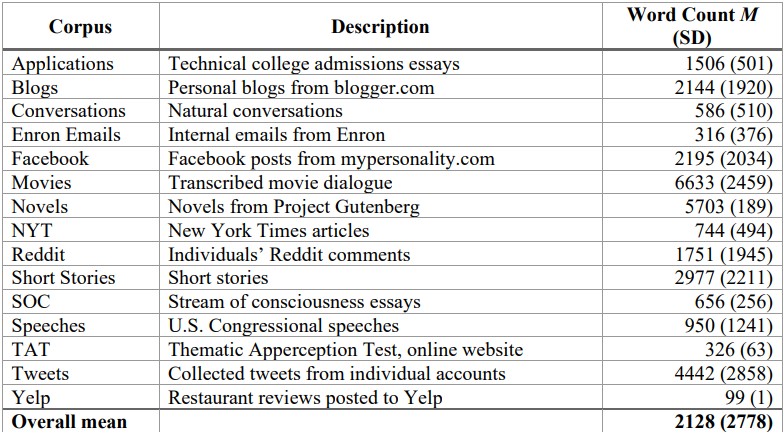
\includegraphics[scale=0.65]{./figures/test-kitchen-corpus.png}
	\caption{The test Kitchen Corpus of 31 Million Words \cite{boyd2022development}}
	\label{FigKitchenCorpus}
\end{figure}

\subsection{Assessing LIWC-22's Accuracy}

\quad The process of quantifying the reliability and validity of text analysis tools like LIWC-22 presents unique challenges, different from the conventional approaches used in psychological assessments. The differences between verbal behavior and structured questionnaire responses needs a nuanced approach to evaluating the properties of LIWC categories.

Unlike self-report questionnaires that measure emotions like anger, sadness or ability to cooperate, through multiple, similar questions to ensure internal consistency, natural language does not conform to such repetitive patterns. In real-world communication, be it a social media post, an essay, or a conversation, individuals express a thought and then naturally progress to the next. This characteristic of verbal expression implies that the standards applied to language-based analyses must be adjusted to account for the unique dynamics of verbal behavior \cite{boyd2022development}.

The evaluation of LIWC-22's reliability involves an innovative adaptation to the language's non-repetitive nature. Taking the LIWC-22 Anger scale as an instance, the scale encompasses 181 words and phrases associated with anger. Theoretically, the usage of one anger-related word in a text should correlate with the usage of other anger-related words within the same text. By analyzing how each of these words is employed across a selection of texts and calculating the intercorrelations among these word usages, LIWC-22's approach to determining internal consistency emerges\cite{boyd2022development}.

Validating the numerous LIWC dimensions poses a significant and complex challenge. By their nature, LIWC's content categories appear to be directly relevant or face valid. Yet, the deeper question lies in determining the extent to which both personal and social psychological processes are mirrored in the use of language. For instance, the implications of using words related to "affiliation" at a high frequency raise questions about the user's social connections and needs. Are individuals using these words seeking more social interaction, or do they reflect a person's existing strong social ties? Additionally, it is important to consider whether the frequency of such language usage offers insights into or predictions about someone's social relationships and needs.

To compute these metrics, LIWC-22 employs two statistical methods: the Cronbach’s alpha (\textalpha) for continuous data, based on the percentage of total words, and the Kuder–Richardson Formula 20 (KR-20) for binary data \cite{kuder1937theory}, indicating the presence or absence of words. The application of Cronbach’s alpha in the context of LIWC-22 encounters a problem due to the variable base rates of word usage within language categories. This variability can lead to underestimations of reliability when using traditional methods. Conversely, the Kuder–Richardson Formula 20 offers a more accurate reflection of a category's internal consistency by accommodating the binary nature of word presence, thus providing a better approximation of reliability in language analysis.

In 2021, there was a great amount of research combining text analysis and social and psychological behaviors, with more than 2,400 studies using LIWC to examine text. Findings from these studies, including those from the developers' own laboratories, reveal correlations between the affect or emotion categories detected by LIWC in texts and the authors' self-reported feelings. These correlations, although modest, show the tool's capability to capture psychological dynamics to a certain extent. Higher correlations are observed when comparing judges' ratings of writing samples with LIWC scores, suggesting a somewhat consistent external validation of LIWC's analytical output\cite{boyd2022development}.

\section{Tokenization for LIWC-22 Compatibility}

\quad We shall delve into the tokenization method utilized in our study, designed to preprocess text data to ensure it aligns with the requirements of the Linguistic Inquiry and Word Count (LIWC-22) tool \cite{boyd2022development}. LIWC requires input texts to be broken down into tokens, a process that can significantly influence the accuracy and reliability of the linguistic analysis. Our chosen methodology leverages the strengths of BERT's tokenization system, as described in the referenced study \cite{bertTokenizerEnglish}.

BERT, or Bidirectional Encoder Representations from Transformers, introduces a sophisticated approach to tokenization that we adapted for our needs. BERT’s tokenization algorithm is based on WordPiece \cite{wu2016google}, handling the input text by initially breaking it down into tokens, which are then further divided into sub-tokens. This mechanism allows for a fine-grained understanding of language, capturing nuances by analyzing tokens in the context of their surrounding text.

The BERT model is pre-trained on a vast corpus of text, allowing it to understand a wide range of linguistic nuances. Its bidirectional nature means that each token is influenced by the tokens that come before and after it, providing a rich context for each word. This context is crucial for accurate linguistic analysis, as the meaning of a word can change significantly depending on its context \cite{bertTokenizerEnglish}. For example, in the sentence “I read that book,” the tokenization process needs to understand whether "read" is in the past or present tense, which has implications for the psychological constructs that LIWC-22 might extract.

By using BERT's tokenization, we ensured that our model could handle the complexity of the text data typically found on platforms like Reddit. This is particularly important for detecting signs of depression, where context can change the sentiment or meaning of a word. Furthermore, the sub-token approach allowed us to maintain the granularity needed for LIWC-22 \cite{boyd2022development}, which often relies on the detection of specific words and categories relevant to psychological states.










\chapter{Model Selection and Hyperparameter Tuning: Optimizing AI for Depression Detection}

\label{chap:ch3}

\quad In the quest to develop an effective AI system for detecting depression from textual data, the choice of the right model and the fine-tuning of its parameters emerge as critical steps. This chapter delves into the intricate process of selecting Random Forest as the preferred model for our task. Known for its robustness and ability to handle complex datasets, Random Forest stands out as a powerful tool in the landscape of machine learning algorithms. However, the journey from selection to optimization is nuanced, involving a series of strategic decisions aimed at enhancing the model's performance.

\section{The Strategic Choice of Random Forest for Depression Detection}

In the ever-expanding realm of machine learning, selecting the most appropriate algorithm is paramount to the success of any predictive modeling task. This is particularly true in the domain of depression detection, where the complexity and variability of the data demand an approach that is not only accurate but also robust and interpretable. Drawing upon the findings of a comprehensive study that evaluated twelve distinct machine learning algorithms across seven datasets\cite{siraj2023performanceModelComparison}, we anchored our decision to employ Random Forest (RF) as the cornerstone of our analysis.

The study \cite{siraj2023performanceModelComparison} in question meticulously compared the performance of several algorithms, including Naive Bayes (NB), Linear Discriminant Analysis (LDA), Logistic Regression (LR), Artificial Neural Networks (ANN), Support Vector Machines (SVM), K-Nearest Neighbors (K-NN), Hoeffding Tree (HT), Decision Tree (DT), C4.5, Classification and Regression Tree (CART), Random Forest (RF), and Bayesian Belief Networks (BB), across multiple metrics. Among these, Random Forest emerged as the clear frontrunner, exhibiting superior accuracy, precision, and Matthew’s Correlation Coefficient (MCC). Following Random Forest, the algorithms of Neural Networks (NN), Naive Bayes (NB), Bayesian Belief Networks (BB), and Logistic Regression (LR) were identified as the next most effective, in descending order of accuracy.

The study \cite{siraj2023performanceModelComparison} also highlighted the significance of the kappa statistic and Root Mean Square Error (RMSE) as vital factors in assessing model performance, further validating the robustness of Random Forest in handling diverse and complex datasets. Inspired by these compelling insights, and in alignment with the study’s conclusion, our selection of Random Forest is underpinned by its demonstrated efficacy across multiple evaluative dimensions.

The datasets utilized for the comparative study are varied, each with its unique characteristics and relevance to different classification tasks:
\begin{itemize}
 
\item Breast Cancer Wisconsin (Original): This dataset contains 11 attributes and is used for binary classification (two classes) with 699 instances. It does include missing values, which would require additional preprocessing steps.

\item Statlog (Vehicle Silhouettes): Comprising 19 attributes over 846 instances, this dataset is for multiclass classification with four distinct classes and has no missing values.

\item Vertebral Column: With 7 attributes and 310 instances, this dataset is also used for multiclass classification, distinguishing among three classes, without any missing values.

\item Breast Tissue: This dataset has 10 attributes across 106 instances and is used for a more complex multiclass classification task with six classes, also free of missing values.

\item Contraceptive Method Choice: It includes 10 attributes and a larger number of instances at 1473. It’s structured for multiclass classification into three classes, and there are no missing values.

\item Image Segmentation: This is a sizable dataset with 20 attributes and 2310 instances for multiclass classification involving seven classes, and it contains no missing values.

\item Artificial Characters: The largest among the datasets listed, it boasts 8 attributes across a substantial 10218 instances. It’s designed for a multiclass classification with ten classes, and like most others here, it lacks missing values.

\end{itemize}

In the context of our study focused on depression detection, our model resembles the Breast Cancer Wisconsin dataset, because we are also tackling a binary classification problem. However, our model differentiates itself with a higher dimensionality, processing 64 input attributes, which poses a greater complexity in feature representation and selection. (Random Forest) RF achieved the highest accuracy at 97.85\%, suggesting it was the most successful in correctly identifying cases of breast cancer. It also topped the charts with the highest kappa value of 95.03\%, indicating a strong agreement between the predictions and the actual classifications. Precision with RF was outstanding as well, hitting a high of 98\%, while its recall was nearly as impressive at 97.9\%, underscoring its ability to identify most of the positive cases. 

Across the rest of the datasets analyzed in the study \cite{siraj2023performanceModelComparison}, Random Forest (RF) consistently delivered standout performance. Its F-measure and Matthew's Correlation Coefficient (MCC) values were notably high, often outperforming other algorithms. For instance, RF attained an accuracy of 98.48\%, kappa value of 98.23\%, and precision and recall rates both at 98.5\% on certain datasets, alongside an exceptional specificity of up to 99.7%.

While K-NN and Logistic Regression (LR) also demonstrated strong performances in certain cases, with K-NN leading in precision and recall in the Breast Tissue dataset and LR excelling with the highest MCC values for the Vehicle and Vertebral Column datasets, RF's overall dominance was clear. RF's ability to achieve the lowest error rates, coupled with the lowest root mean square error in the majority of datasets, further confirms its robustness and reliability as an algorithm for complex predictive tasks, including depression detection.

In summary, the numerical evidence from the study \cite{siraj2023performanceModelComparison} underlines RF's superior ability to handle complex predictive tasks, making it the algorithm of choice for our model aimed at accurately detecting depressive patterns within textual data.



\chapter{AI Model for Romanian Language}
\label{chap:ch4}
\par \quad Multilingual depression detection is highly dependant on the capability of AI models to understand and analyze text from different cultures. This section describes the process of translating English text into Romanian, a step essential for training our AI model to recognize depressive patterns in a multilingual context. We will discuss the selection criteria and the impact of utilizing a specific Translation API to bridge the language gap, thus enabling our model to process and interpret Romanian text with the same level of accuracy as English. 

\section{Reasoning Behind Choosing Yandex}

\quad In our effort to refine our multilingual depression detection model, we referenced a detailed study that assessed the efficiency, accuracy, and security of various Translation APIs \cite{rashmi2020comparison}. This comparative analysis served as the foundation for selecting the most suitable API for our application, which required the translation of text from English to Romanian among other language pairs. The study meticulously compared several leading Translation APIs, including Google API, Microsoft, Systran.io, MyMemory, and Yandex, focusing on their performance in terms of speed, accuracy, security, and the breadth of language support.
\begin{itemize}
\item \textbf{Google API} is widely recognized for its impressive language support, capable of translating content across more than 100 languages. This extensive reach makes it a versatile tool for global communication and content translation. Its reputation and prevalence in the market are testaments to its utility and user-friendly interface. Additionally, it's worth noting that while Google API is commendable, it is not a free service, which may affect its accessibility for some users.\cite{rashmi2020comparison}.

\item \textbf{Microsoft's Translation API} is lauded for its quality and security, offering translations among 60+ languages. It stands out for its emphasis on accuracy and stringent security protocols, although its language support is less extensive than Google's \cite{rashmi2020comparison}.

\item \textbf{Systran.io} boasts a high accuracy rate of 99\%, albeit with limitations in recognizing slang, nuances, and culturally relevant phrases. Its security is commendable, positioning it as a reliable choice for many applications \cite{rashmi2020comparison}.

\item \textbf{MyMemory} excels in translation speed but experiences the highest latency among the APIs evaluated. While it supports translations between 80+ languages, the absence of training data for certain language combinations limits its effectiveness. Nonetheless, its security is robust \cite{rashmi2020comparison}.

\item \textbf{Yandex API}, with support for 90+ languages, stands out for its balance of translation accuracy and lower latency compared to its counterparts. Despite its efficiency and broad language coverage, its security features are not optimal for translating confidential documents \cite{rashmi2020comparison}.
\end{itemize}

The conclusion from this study discussed the strengths and weaknesses of each API, guiding our choice towards Yandex API for our multilingual depression detection model. Yandex was selected due to its free access, lower latency, and reliable accuracy across different cultures, making it an ideal tool for everyday translations where security is not the biggest concern \cite{rashmi2020comparison}. This choice aligns with our objective of giving people an easy to use and accessible tool in order to prevent problems that could appear with depression.

Another rigorous study \cite{cambedda2021study} provides a nuanced error analysis of Yandex's translations. Notably, Yandex's performance, depicted in the graph \ref{YandexTranslationPerformance}, indicates a relatively uniform distribution of errors across multiple categories. This suggests that while Yandex does have areas where it lacks consitency, such as Lexis, Syntax, and Article Usage, it generally maintains the core meaning of the translated text. This is critical for our model, which relies on emotion categories to accurately detect depression in text.

\begin{figure}[htbp]
	\centering
		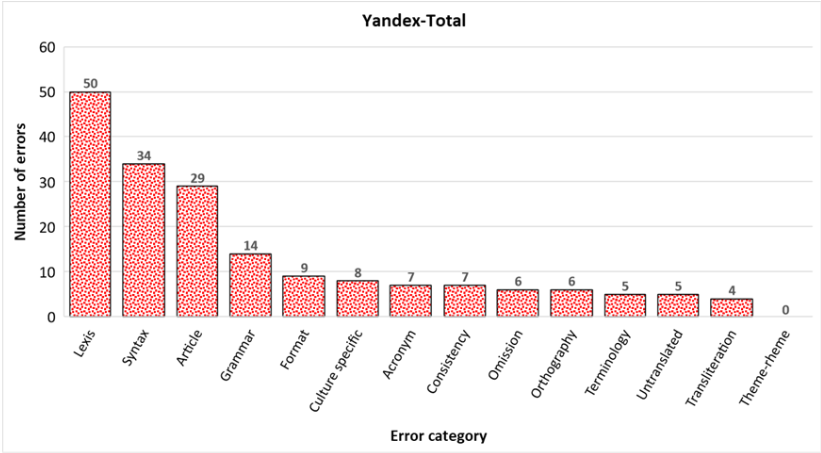
\includegraphics[scale=0.65]{LaTeX Bachelor Thesis Depression Signs Detection/figures/Yandex's-translation-performace.png}
	\caption{Yandex's translation performance \cite{cambedda2021study}}
	\label{YandexTranslationPerformance}
\end{figure}

The Lexis category, in particular, displays the highest number of errors, signaling a need for further investigation to understand whether these issues are from the nature of the texts or from challenges within the translation tool. However, it is encouraging to note that error categories such as Grammar, Format, Culture-Specific References, Acronym, and Consistency show significantly fewer errors. These categories are essential for maintaining the general meaning, which reaffirms our choice of Yandex for texts where nuanced meaning is less likely to affect the detection of depression signs.

Further examination of the study indicates that Yandex demonstrates a more adept handling of common language texts as opposed to those with specialized jargon, registering fewer errors in translations of texts with language spoken by the people in a particular country or region \cite{cambedda2021study}. Considering our dataset comprises of Reddit posts, which are typically phrased in everyday language, this finding is particularly relevant. The study also highlights that, with the exception of Article Usage, the disparity in error rates between different text types is negligible, suggesting that Yandex can reliably manage the conversational and informal style characteristic of Reddit communications.

\section{Adjusting to Yandex API's Policy Shift}

\quad We had initially recognized the Yandex API as a superior option, particularly for its cost-effectiveness, as it was freely accessible at the time of study \cite{rashmi2020comparison}. This advantage aligned with our objectives, allowing us to use its translation capabilities without financial constraints.

However, since the publication of \cite{rashmi2020comparison}, Yandex's policy has undergone significant changes. The API, once free to use within a given generous limit, now requires users to possess a registered and legally recognized company to utilize its services. Ihe requirement of company registration introduces a barrier, limiting the accessibility of Yandex API for independent researchers, small teams, or educational institutions.

Given these new rules, we are still fully dedicated to creating a useful and easy-to-use depression detection system that works in many languages. Therefore, we are looking into different approaches.

\section{Shifting to googletrans}

\quad We decided to integrate the googletrans library \cite{googletranslib} into our multilingual depression detection model. It offers a free and unlimited Python library that uses the Google Translate API. This library appears particularly advantageous for our requirements, as it is not only accessible without cost but also does not require the a company registration that Yandex now demands. As it can be seen in \ref{codeGoogleTransUsage}, it is very accessible to translate text in Python from English ro Romanian.

\begin{figure}[htbp]
	\centering
		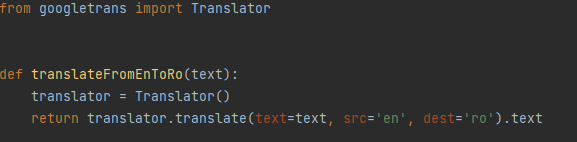
\includegraphics[scale=1]{LaTeX Bachelor Thesis Depression Signs Detection/figures/codeGoogleTransUsage.png}
	\caption{Python library "googletrans" translation from English to Romanian}
	\label{codeGoogleTransUsage}
\end{figure}

The googletrans library \cite{googletranslib} has features that are well-suited to our project's needs. It is recognized for its speed and reliability, as it operates on the same servers as translate.google.com. The library supports auto language detection, facilitating the identification and translation of a wide array of languages without prior specification. Additionally, it provides the capability for bulk translations, which is invaluable when processing large datasets typically found in NLP tasks. It was done for the chosen dataset \cite{depressionDataset} in Python as it can be seen in \ref{codeDatasetTranslation} .

\begin{figure}[htbp]
	\centering
		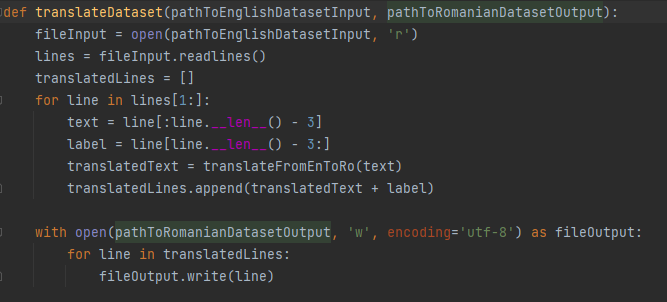
\includegraphics[scale=1]{LaTeX Bachelor Thesis Depression Signs Detection/figures/codeDatasetTranslation.png}
	\caption{Python code for translating dataset from English to Romanian}
	\label{codeDatasetTranslation}
\end{figure}

It is also important to acknowledge googletrans's \cite{googletranslib} usage notes. The 15,000-character limit per text may require segmentation of longer entries, and the instability of web-based translation services means that we should proceed with precaution regarding the library's reliability. The developers themselves suggest opting for the official Google Translate API for more advanced applications where stability is very important. Furthermore, potential HTTP errors could indicate temporary bans by Google, meaning that it is needed to keep an eye on and manage how we use our API to avoid any interruptions. Despite these considerations, the googletrans library's free and flexible usage makes it an excellent fit for our project in its current stage.

\section{Model Training}

\quad For the Romanian language model, the methodology was replicated consistently. LIWC served as the tool for preprocessing the data. However, the most recent English dictionary for LIWC-22 has not been translated into Romanian. The latest available version for Romanian is the LIWC-2015 dictionary, which contains only 86 features, compared to the 119 features available in the English version.

The training approach was aligned with the methodology used for the English model during the second experiment. The hyperparameters and the proportion of training to testing data remain consistent:

\begin{itemize}
\item \textbf{train/test split}: Maintained at 75/25, using stratification based on the 'is\_depression' label
\item \textbf{mtry}: 6
\item \textbf{Number of trees}: 900
\item \textbf{Node Size}: 3
\item \textbf{Sample size}: 8
\end{itemize}

This methodology facilitates a direct comparison between the performance of the Romanian and English models, ensuring consistent evaluation criteria across both. The same metrics were used for analysis. In terms of classification metrics, the most notable discrepancy arises in recall, where the Romanian model scores 0.87, falling short of the English model's 0.96 by 9 percentage points. Additionally, both accuracy and the F1-score have diminished by 0.05, while precision experienced the least impact, decreasing from 0.99 to 0.97. These metrics are illustrated in Figure \ref{classificationMetricsSecondExperiment} for the English model and in Figure \ref{classificationMetricsRomanianExperiment} for the Romanian model.

The diminished recall in the Romanian model suggests it is less adept at identifying true positive cases as compared to the English model. This lower performance may come from the nuances lost during the translation of the dataset from English to Romanian using the Googletrans library \cite{googletranslib}. Such translation challenges could contribute to the model’s reduced effectiveness, highlighting the influence of linguistic or cultural differences on the model’s ability to generalize across languages. The smaller reductions in accuracy and F1-score indicate that while the model is somewhat less effective overall, it still maintains a reasonable level of precision.

\begin{figure}[htbp]
	\centering
		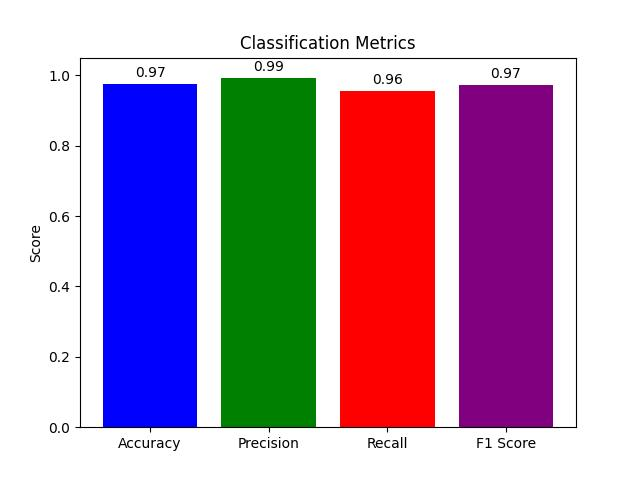
\includegraphics[scale=0.8]{LaTeX Bachelor Thesis Depression Signs Detection/figures/metrics/experimentRomanian/classificationMetrics.jpg}
	\caption{Classification Metrics Romanian Model}
	\label{classificationMetricsRomanianExperiment}
\end{figure}

The confusion matrix \ref{confusionMatrixRomanianExperiment} illustrates a significant increase in false positives, rising from 43 in the English model \ref{confusionMatriSecondExperiment} to 123 in the Romanian model. However, the rise in false negatives was less marked, increasing from 7 to 26.

\begin{figure}[htbp]
	\centering
		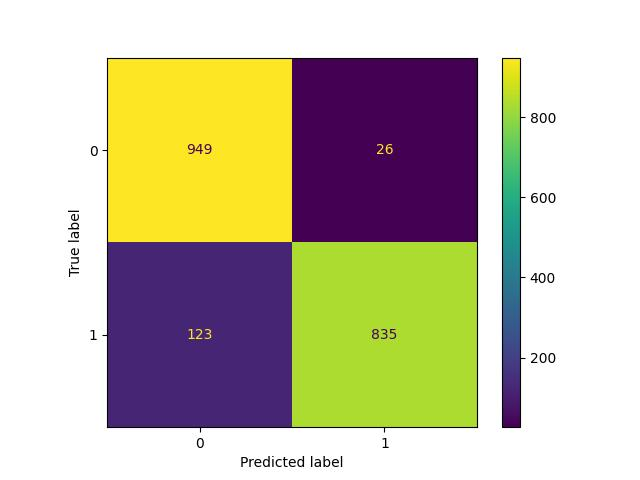
\includegraphics[scale=0.8]{LaTeX Bachelor Thesis Depression Signs Detection/figures/metrics/experimentRomanian/confusionMatrix.jpg}
	\caption{Confusion Matrix Romanian Model}
	\label{confusionMatrixRomanianExperiment}
\end{figure}

Regarding the ROC curve, the Area Under the Curve (AUC) experienced a slight decrease of 0.01, as depicted in Figure \ref{rocCurveRomanianExperiment} compared to Figure \ref{rocCurveSecondExperiment}. These metrics collectively indicate that the issues observed during the experimentation with the English model are more pronounced in the Romanian classifier.

\begin{figure}[htbp]
	\centering
		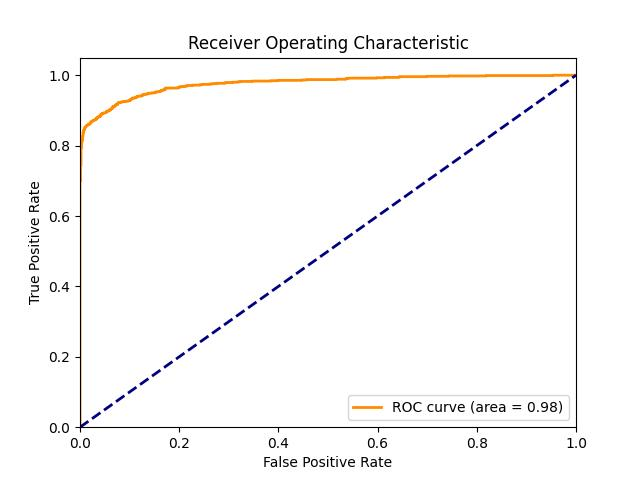
\includegraphics[scale=0.8]{LaTeX Bachelor Thesis Depression Signs Detection/figures/metrics/experimentRomanian/roc_curve.jpg}
	\caption{ROC Curve Romanian Model}
	\label{rocCurveRomanianExperiment}
\end{figure}

The most significant features for the Romanian classifier \ref{top10FeaturesRomanianExperiment} align more closely with those observed in the initial experiment for the English model \ref{top10FeaturesFirstExperiment}. Notably, Word Count (WC) has risen above 0.12, surpassing the prominence it held in the first experiment. This contrasts with the enhancements seen in the second English experiment \ref{top10FeaturesSecondExperiment}, where a diminished reliance on WC and WPS (Words per Sentence) indicated a broader array of features influencing the English classifier’s decisions. However, this diversification does not appear to extend to the Romanian model.

Some features remain consistent with the English LIWC-22 dictionary features listed in the top 10 for the second experiment; for instance, "sad" aligns with "emo\_sad", and both "cause" and "health" are both present and "negemo" is the same as "emo\_neg". The "anx" feature mirrors "emo\_anx" from the first experiment’s top features. The presence of "Period" suggests that the Googletrans library has introduced punctuation marks, which have become a significant element. The evolution from LIWC-2015 to LIWC-22 is further evidenced by the removal of the "interrog" category in the Romanian model’s top 10 features, which was dropped in LIWC-22 due to its low base rates, internal reliability, or infrequent usage, as noted in \cite{boyd2022development}. The "ipron" feature might also result from the machine translation process.

\begin{figure}[htbp]
	\centering
		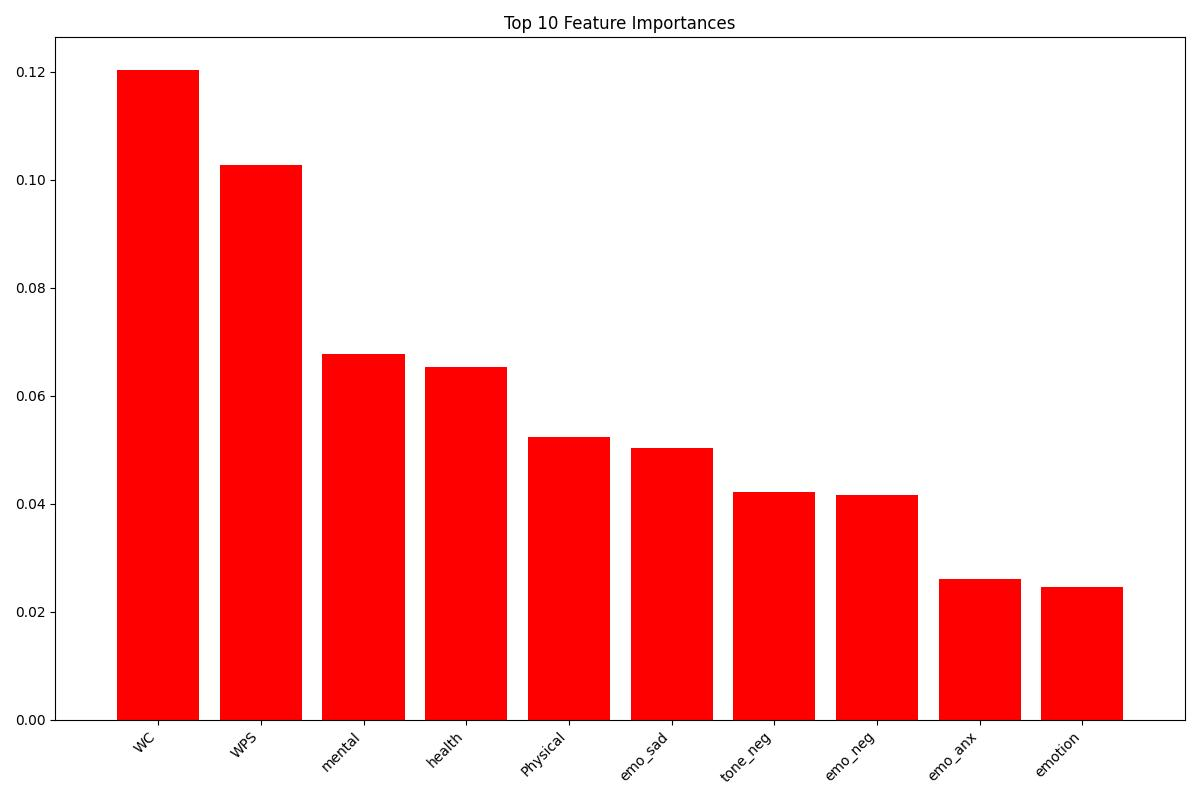
\includegraphics[scale=0.5]{LaTeX Bachelor Thesis Depression Signs Detection/figures/metrics/experimentRomanian/top10features.jpg}
	\caption{Top 10 Features Romanian Model}
	\label{top10FeaturesRomanianExperiment}
\end{figure}

\chapter{Conclusions and Future Work}
\label{conclusions}

\quad Developing a multilingual tool presents significant challenges. There is a much richer body of literature for English than for Romanian, which impacts the performance of AI models, as evidenced by our experiments. The English model achieved a precision of 96\%, significantly higher than the Romanian model's 87\%. This difference largely comes from the translation methods used and the limitations of the pre-processing tool LIWC. Despite using Google Translate, a leading translation service, the Googlelib \cite{googletranslib} encountered difficulties in maintaining the original text's meaning. Additionally, the most recent version of LIWC, LIWC-22, is only available in English, which meant a downgrade to LIWC-2015 for Romanian, which is seven years behind in advancements, as reflected in the precision of our Romanian classifier.

For future improvements, employing an AI-based translation tool could preserve text meaning more effectively. Also, since LIWC \cite{boyd2022development} specifies its use strictly for academic purposes, any commercial application would need to adopt a different pre-processing approach to cover licensing costs. Such advancements could greatly aid in targeted marketing for psychologists or enhancing mental health awareness, aligning with the goals of the "Depression Signs Detector" tool. The next step for the tool is its deployment to a production environment, transitioning from localhost to a cloud hosting platform to ensure broader accessibility and reliability.

As a computer science researcher, I cannot provide human-based validation for diagnosing depression, such validation must be performed by a specialist. Unlike object detection in images, which can be visually verified by nearly anyone, assessing the accuracy of depression detection outputs is beyond a programmer’s capability.

Moreover, while communicating, words represent only a minor fraction of the information conveyed. The tool, which solely analyzes text, is insufficient to conclusively determine if a person is depressed. Therefore, it is important to note that the tool serves merely as a preliminary assessment of a person’s emotional state, a thorough evaluation requires a professional in psychology. For a more accurate computer-based analysis, it would be necessary to consider all aspects of communication, both verbal and nonverbal.


%\addcontentsline{toc}{chapter}{Concluzii}
%\addcontentsline{toc}{chapter}{Conclusions}

\bibliography{references}

\end{document}
%TODO: cand cumpar licenta pt liwc schimbat inloc de 64 input attributes cu cate o sa am